%%% Results %%%
\chapter{Results} \label{ch:results}
This chapter evaluates the result of endorsement model as presented in section
~\ref{ch:method} by using interaction graph on existing dataset. Results will
be presented along with the discussion of measurement metrics and analyzed to
see if the requirements mentioned in section ~\ref{ch:UserStories} are met.  
%%%%%%%%%%%%%%%%%%%%%%%%%%%%%%%%%%%%%%%%%%%%%%%%%%%%%%%%%%%%%%%

%%%%%%%%%%%%%%%%%%%%%%%%%%%%%%%%%%%%%%%%%%%%%%%%%%%%%%%%%%%%%%%
\section{Interaction graph}
In order to simulate the interaction graph, existing dataset from SNAP
\cite{snapnets} was used. The dataset was extracted from Bitcoin Alpha trust
\footnote{https://alphabtc.com/blockchain/} weighted signed network which was
essentially a who-trusts-whom network of people that trade on Bitcoin Alpha
platform. Participants on this network rated each other on a scale of -10 to
+10 where negative value represented total distrust whereas positive value
represented total trust. It consists of 3,783 nodes that made 24,186 edges out
of which 93\% of the edges were marked as positive edges\cite{kumar2016edge}.\\
\begin{figure}[h]
	\includegraphics[width=0.95\textwidth]{Images/in_out.eps}
	\caption{Given Vs. Received}
	\label{inOut}
\end{figure}
The available information in the dataset for all the nodes was source, target,
rating, and timestamp. All of which is essential information for endorsement
network. The direction of endorsement is based on the source and target
information. The timestamp is also essential information if using a network
anomaly detection algorithm such as net flow rate convergence(cite). The rating
shows the strength or weakness of the relation. For the endorsement relation,
only the edges with a rating above two are considered. Thus, the total number
of nodes considered for endorsement interaction was 1677.\\ 
\textbf{nEG and nER:} nEG and nER is outdegree and indegree information
respectively.  The distribution of which can be seen in figure ~\ref{inOut}.
As mentioned in the requirement(req.no), each node needs to have at least 2 or
more connections to be considered for impact computation. Failing to do so
would result in an impact value equivalent to zero. Of the 1677 nodes in the
network, there were 1175 nodes(70\%) that had only one incoming or outgoing
connection. As a result, only 502 nodes(30\%) can have an impact above zero.\\ 

\begin{tabularx}{\textwidth}{| X | X | X | X | X| X| }
  \hline
   \textbf{Node Label} & \textbf{nEG} & \textbf{nER} & \textbf{ratio} & \textbf{ReceivedPoints} & \textbf{Impact} \\
  \hline 
  430  & 5  & 3  & 0.6 & 0 & 0 \\
  \hline
   761 & 2  & 2  & 1 & 0 & 0 \\
  \hline
  448  & 3  & 3  & 1 & 0 & 0 \\
  \hline
  676  & 2  & 2  & 1 & 0 & 0 \\
  \hline
  936  & 2  & 2  & 1 & 0 & 0 \\
  \hline
  \caption{Nodes with Impact zero because of the receivedpoints}
  \label{table:receivedpoints}
\end{tabularx}

\textbf{Received Points:} The total received point plays an equally significant
role in strengthening or weakening the total endorsement impact of a node. This
factor relies on the significance of node from whom one receives the
endorsement. Table ~\ref{table:receivedpoints} shows the nodes that have a
maintained ratio of connections but still have zero impact on the network
because of the total received points. As can be seen in figure
~\ref{fig:zeroimpact}, the endorser of nodes 430, 761, 448, 676 and 936 has no
other connection in the network. Therefore, these nodes have an impact of zero
just like their endorsers. The relation of total received point and its
contribution to the endorsement impact can be seen in figure
~\ref{fig:receivedpointvsimpact}.
\begin{figure}[h]
	\includegraphics[width=0.95\textwidth]{Images/receivedPoints_impact_impactAboveZero.eps}
	\caption{Received Points Vs. Total Endorsement Impact}
	\label{fig:receivedpointvsimpact}
\end{figure}


\begin{figure}[h]
	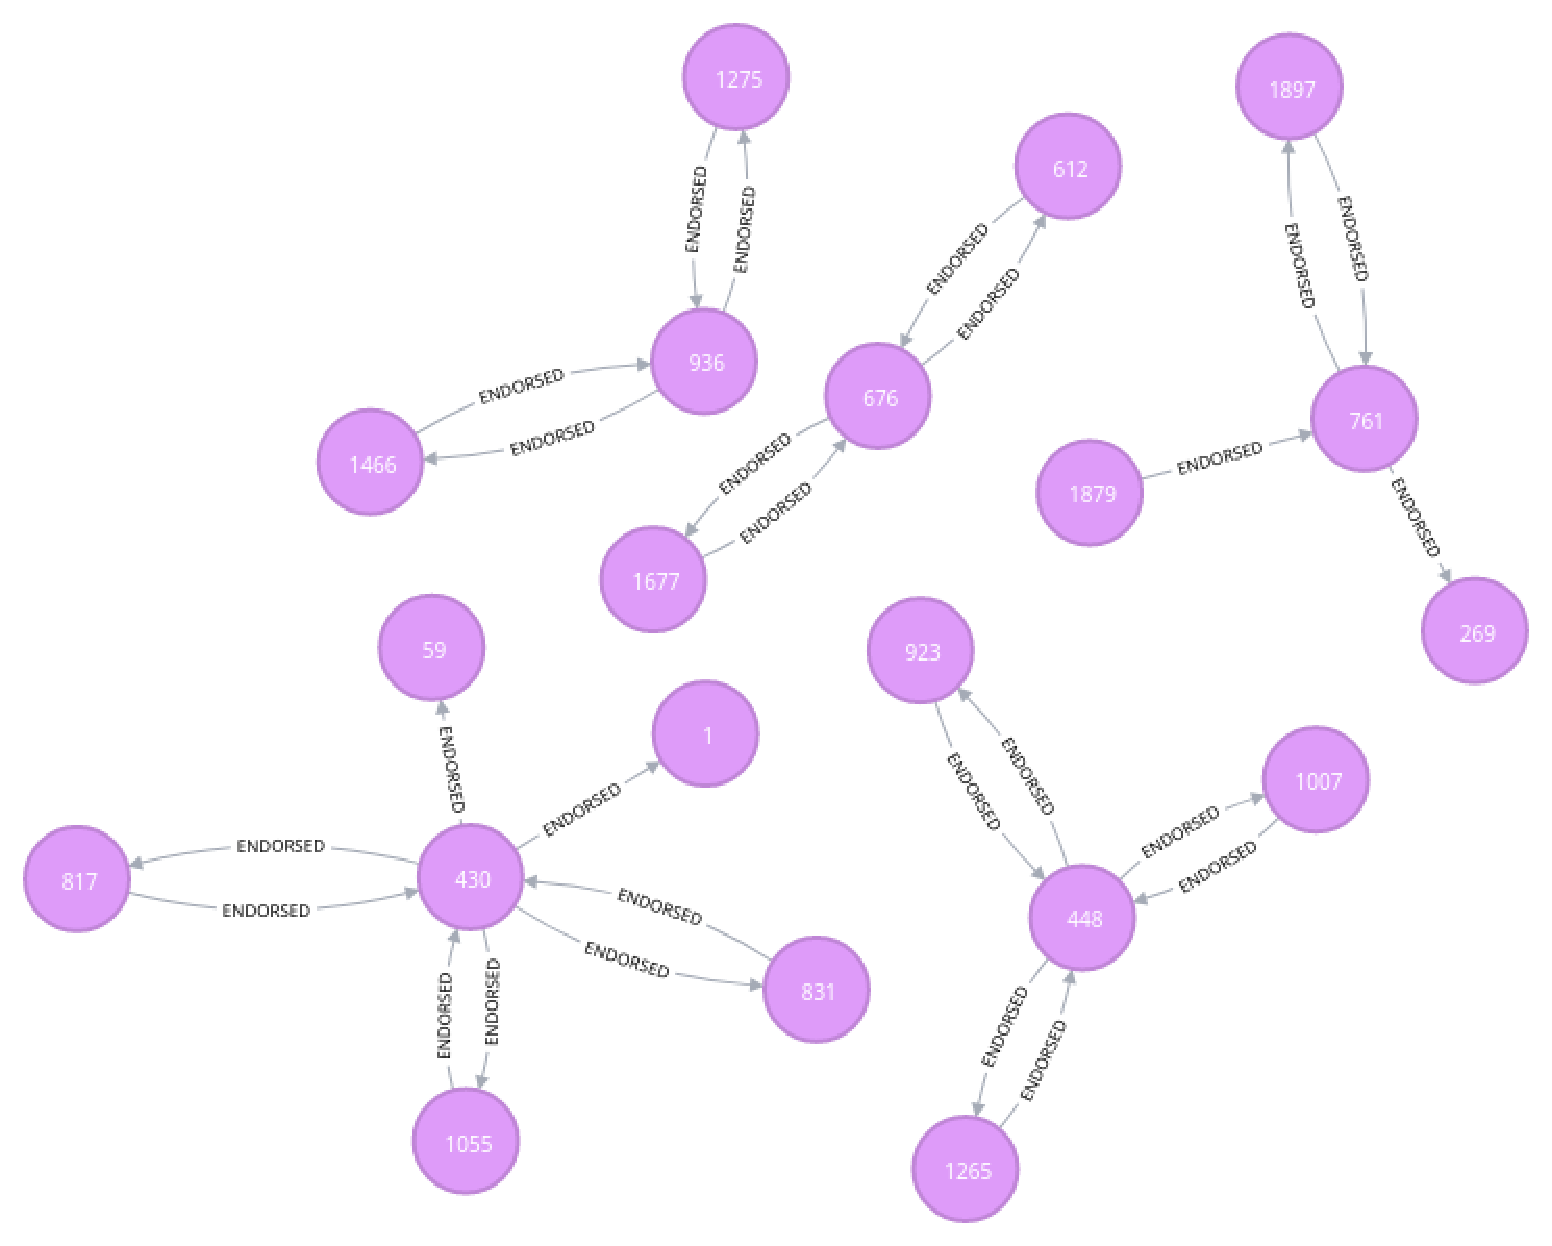
\includegraphics[width=0.95\textwidth]{Images/nodesWithImpactZero.eps}
	\caption{Interaction subgraph of nodes with impact zero}
	\label{fig:zeroimpact}
\end{figure}
\textbf{Total Endorsement Impact:} The endorsement impact in this model alone
is affected by the received point and the degree of connections. For the given
network, the majority of the nodes have an impact value below 20. There are
however few nodes that have managed to obtain an impact value above 100. Each
of the nodes having both maximum and minimum impact value is discussed across
four scenarios in the section that follows.  The distribution of the obtained
impact ranges and the number of nodes are presented in table
~\ref{table:totalimpact}.

\begin{tabularx}{\textwidth}{| X | X | }
  \hline
   \textbf{No. of nodes} & \textbf{Impact Range} \\
  \hline 
  419  & 0-5  \\
  \hline
   51 & 5-10 \\
  \hline
  5 & 10-15 \\
  \hline
  10 & 15-20 \\
  \hline
  2 & 20-25 \\
  \hline
  1 & 25-30 \\
  \hline
  1 & 30-35 \\
  \hline
  0 & 35-65 \\
  \hline
  1 & 65-70 \\
  \hline
  0 & 70-85 \\
  \hline
  2 & 85-90 \\
  \hline
  0 & 90-115 \\
  \hline
  1 & 115-120 \\
  \hline
  3 & 120-125 \\
  \hline
  0 & 125-150 \\
  \hline
  1 & 150-155 \\
  \hline
  \caption{No. of nodes and the corresponding impact ranges}
  \label{table:totalimpact}
\end{tabularx}

\begin{figure}[h]
	\includegraphics[width=0.95\textwidth]{Images/ratio_impact_impactAboveZero.eps}
	\caption{Relation of Ratio and Total endorsement impact}
	\label{fig:ratioimpact}
\end{figure}

\section{Impact and Ratio: Case-by-case across different scenarios}
The representation in table ~\ref{table:receivedpoints} and figure
~\ref{fig:ratioimpact}, points that maintaining a ratio of 1 or close to 1 is
not enough to have a higher impact on the endorsement network. One can infer
that having a good impact implies a good ratio but having a good ratio does not
necessarily imply a good impact.
As such, a case-by-case analysis for the possible combination of ratio and
impact is performed. The maximum value for the impact, ratio, nEG, nER and
received points is the maximum value found in the network for the respective
variables.The nodes with impact value in the range of 0-15 are taken as low
impact nodes, and value above 100 is taken as high impact node for the
scenarios.   
\begin{itemize}
	\item Case1: Maximum Impact/Minimum Ratio: If a user has been on the network
		for a while making endorsement connections, then it is possible to have
		a higher impact. Since receiving an endorsement from many connections
		cumulative sums up to the existing value. The higher received point, in
		this case, contributes to the higher impact. The behavior as depicted
		in figure ~\ref{fig:case1} is extracted from the endorsement network among
		the best impact node with a low ratio. 
	\begin{figure}[h]
		\includegraphics[width=0.95\textwidth]{Images/case-1-max-impact-min-ratio.eps}
		\caption{Case1- Maximum Impact Minimum Ratio}
		\label{fig:case1}
	\end{figure}
	\item Case 2: Maximum Impact/Maximum Ratio: A node with a maximum impact
		and a maximum ratio is the best case scenario of endorsement network.
		This scenario implies that a node has been actively participating as
		both endorser and endorsee. The figure ~\ref{fig:case2} shows the
		behavior of such node. The value across all dimension is almost equally
		distributed.  
	\begin{figure}[h]
		\includegraphics[width=0.95\textwidth]{Images/case-2-max-impact-max-ratio.eps}
		\caption{Case2- Maximum Impact Maximum Ratio}
		\label{fig:case2}
	\end{figure}
	\item Case 3: Minimum Impact, Minimum Ratio: A minimum impact along with
		minimum ratio is a sign of node that doesn't have a good
		trustworthiness range. This case generally appears if the node is only
		making one-way connections. i.e., giving too many endorsements and
		receiving none/few or vice-versa. The figure ~\ref{fig:case3} shows
		such behavior. 
	\begin{figure}[h]
		\includegraphics[width=0.95\textwidth]{Images/case-3-min-impact-min-ratio.eps}
		\caption{Case3- Minimum Impact Minimum Ratio}
		\label{fig:case3}
	\end{figure}
	\item Case 4: Minimum Impact, Maximum Ratio: This case has been
		demonstrated earlier by table ~\ref{table:receivedpoints} and figure
		~\ref{fig:ratioimpact}. Figure ~\ref{fig:case4} gives the behavior of
		such a node as seen in the network.
	\begin{figure}
		\includegraphics[width=0.95\textwidth]{Images/case-4-min-impact-max-ratio.eps}
		\caption{Case4- Minimum Impact Maximum Ratio}
		\label{fig:case4}
	\end{figure}
\end{itemize}


%\section{Analysis}
%\section{Measurement}
%\section{Comparison}
%\section{first section} \label{sec:sectionlabel}

% Presentation of results and case-study data 
% An application of the methodology is unfolded and results are presented using for example via Charts, Diagrams, Figures and Tables 
% The work is conducted in accordance with the method described earlier. Results are presented in an analytical way.
